\chapter{Implementacija i korisničko sučelje}
		
		
		\section{Korištene tehnologije i alati}
			 
			 \par
			 Komunikacija u timu realizirana je korištenjem aplikacija \underline{WhatsApp}\footnote{\url{https://www.whatsapp.com/}} i \underline{Discord}\footnote{\url{https://discord.com/}}. Za izradu UML dijagrama korišten je alat \underline{Visual Paradigm Online}\footnote{\url{https://online.visual-paradigm.com/}}. Kao sustav za upravljanje izvornim kodom korišten je \underline{Git}\footnote{\url{https://git-scm.com/}} te je udaljeni repozitorij projekta dostupan na platformi \underline{GitLab}\footnote{\url{https://gitlab.com/}}. Za izradu dokumentacije korišten je softverski sustav za pripremu dokumenata \underline{LaTeX}\footnote{\url{https://www.latex-project.org/}}.
			 \par
			 Kao razvojno okruženje korišteno je integrirano razvojno okruženje Microsofta - \underline{Microsoft Visual Studio}\footnote{\url{https://visualstudio.microsoft.com/}}. Čini ga opsežan skup alata za izgradnju ASP.NET aplikacija, desktop aplikacija i mobilnih aplikacija. Kao urednik izvornog koda za rad na \textit{frontendu} korišten je i Microsoftov uređivač izvornog koda - \underline{Visual Studio Code}\footnote{\url{https://code.visualstudio.com/}}.
			 \par
			 Za izradu \textit{frontend} dijela aplikacije korišten je \underline{.NET Framework}\footnote{\url{https://dotnet.microsoft.com}} te \underline{C sharp}\footnote{\url{https://https://docs.microsoft.com/en-us/dotnet/csharp/}}, dok je \textit{backend} dio aplikacije napravljen koristeći \underline{React}\footnote{\url{https://https://reactjs.org/}} i \underline{JavaScript}\footnote{\url{https://https://www.javascript.com/}}. .Net Framework jest radni okvir razvijen od strane Microsofta koji programerima uvelike pomaže u prevođenju i izvođenju programa. React je besplatna JavaScript biblioteka otvorenog koda za izgradnju korisničkih sučelja.
			 \par
			 Baza podataka nalazi se na poslužitelju u oblaku \underline{Microsoft Azureu}\footnote{\url{https://portal.azure.com/}}. To je računalna platforma koja omogućuje pristup i upravljanje aplikacijama i uslugama. 
			
			\eject 
		
	
		\section{Ispitivanje programskog rješenja}
			
			\subsection{Ispitivanje komponenti}
			

			
			\par
			Svi unit testovi izvršeni su automatski. Ispitivanje je provedeno po serviceima te su se tako provjeravale pojedine komponente sustava. U svakom su testu na početku dohvaćeni DbContext i Mapper.
		
			
			\noindent \textbf{Ispitni slučaj 1: Dohvaćanje svih korisnika}
			
			\noindent \textbf{Ulaz:}
			
			\begin{packed_enum}
				
				\item Stvaranje novog UserServicea
				\item Dohvaćanje metode GetAllUsers
				
			\end{packed_enum}
		
			\noindent \textbf{Očekivani izlaz:}
		
			\begin{packed_enum}
			
				\item Stvara se novi UserService
				\item Dohvaćaju se svi korisnici
				\item Rezultat testa je ispravan
			
			\end{packed_enum}
		
			\noindent \textbf{Izlaz:} Test je zadovoljen. Aplikacija je prošla test.
			
			\begin{figure}[H] 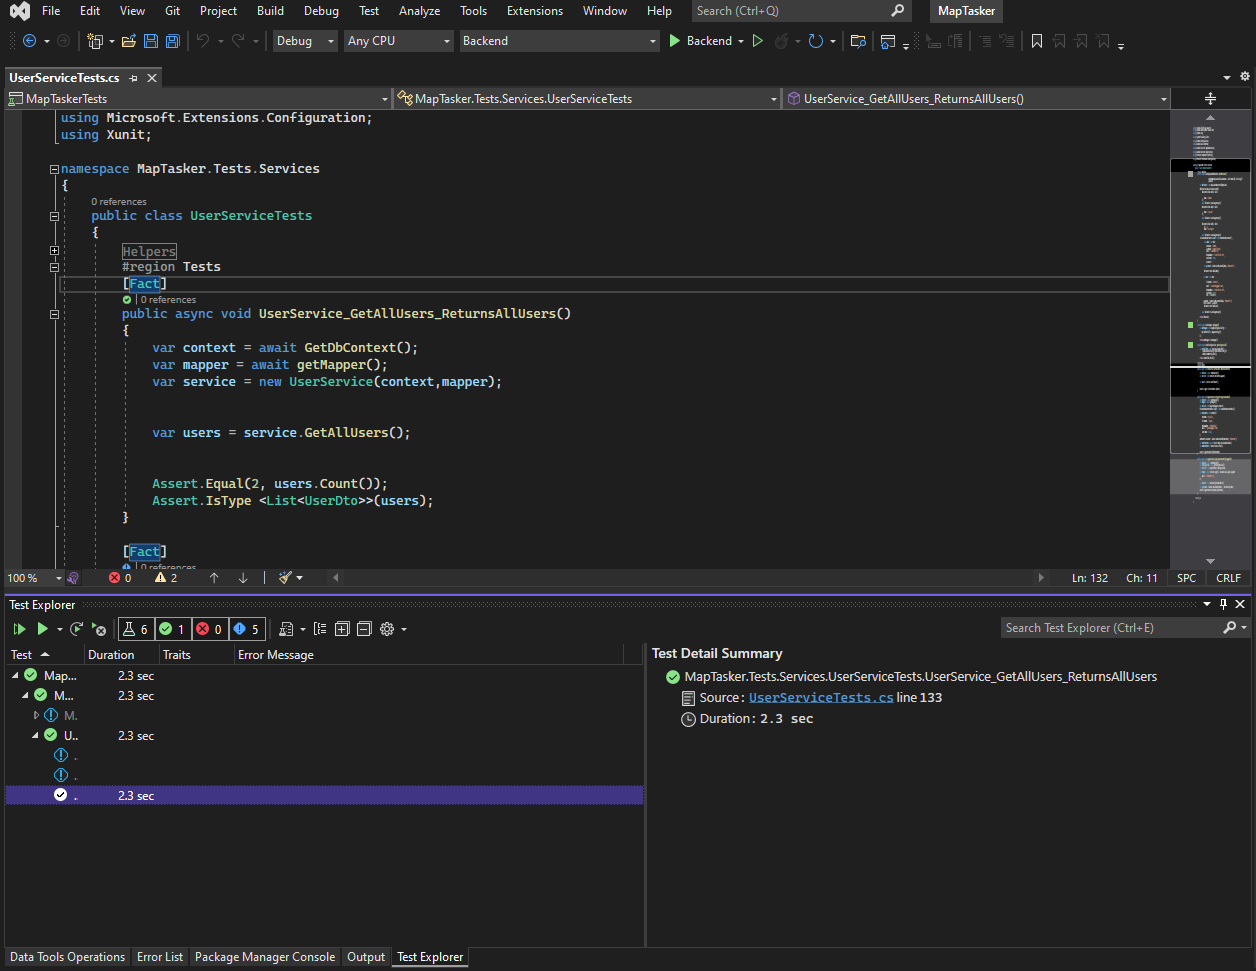
\includegraphics[width=\linewidth]{./slike/Testovi/Unit/UnitTest_1.png}
				\caption{GetAllUsers - ReturnsAllUsers Test}
			\end{figure}
			
			\eject
			
			\noindent \textbf{Ispitni slučaj 2: Uspješna registracija korisnika}
			
			\noindent \textbf{Ulaz:}
			
			\begin{packed_enum}
				
				\item Stvaranje novog RegisterServicea
				\item Kreiranje password hashera
				\item Instanciranje novog korisnika
				\item Postavljanje lozinke korisniku
				\item Dohvaćanje DTO-a Usera i ukupnog broja korisnika za provjeru
				
			\end{packed_enum}
			
			\noindent \textbf{Očekivani izlaz:}
			
			\begin{packed_enum}
				
				\item Stvara se novi RegisterService
				\item Kreira se novi password hasher
				\item Novi korisnik se uspješno stvara
				\item Lozinka se uspješno postavlja korisniku
				\item Rezultat testa je ispravan
				
			\end{packed_enum}
			
			\noindent \textbf{Izlaz:} Test je zadovoljen. Aplikacija je prošla test.
			
			\begin{figure}[H] 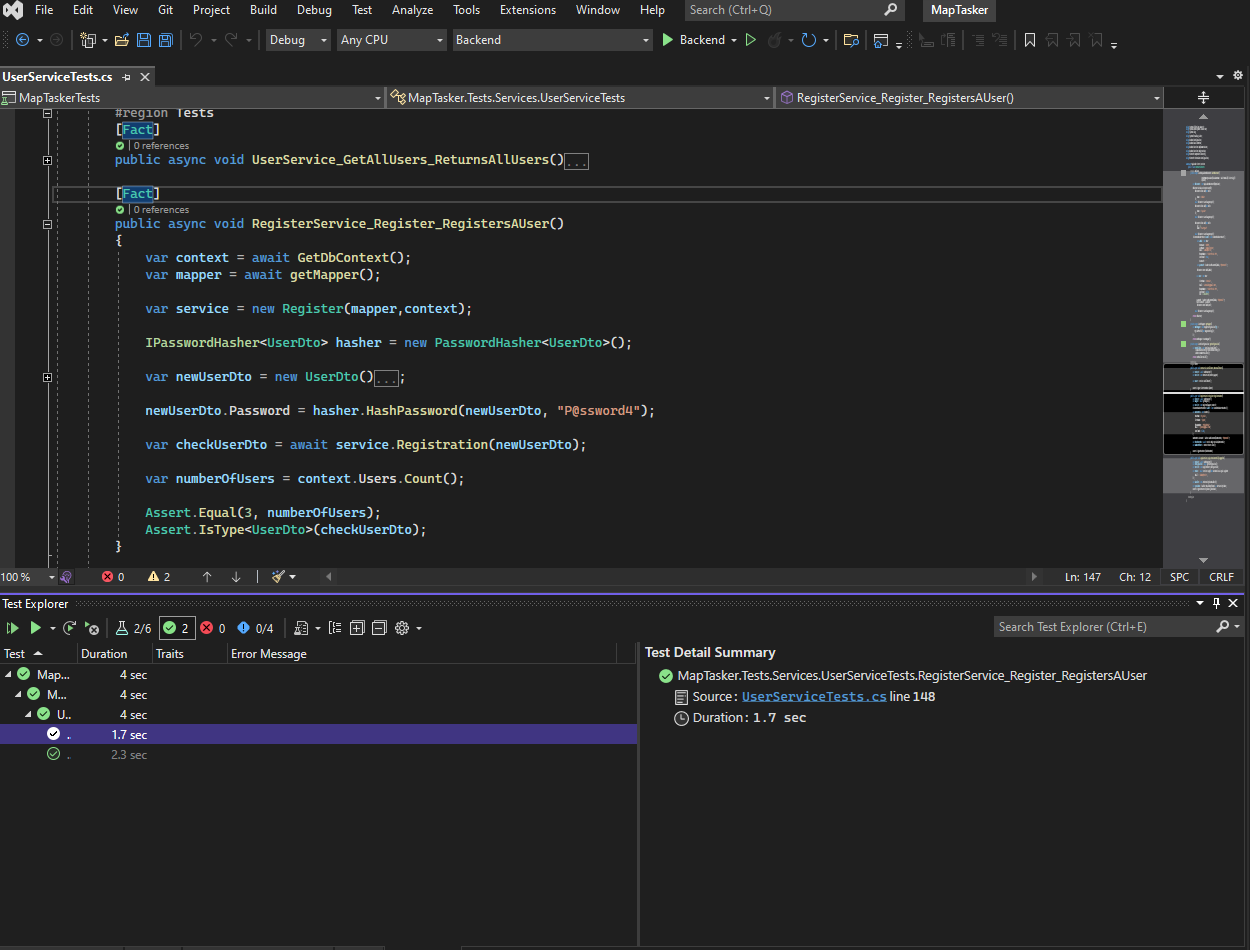
\includegraphics[width=\linewidth]{./slike/Testovi/Unit/UnitTest_2.png}
				\caption{Register - RegistersAnUser Test}
			\end{figure}
			
			\eject
		
			\noindent \textbf{Ispitni slučaj 3: Uspješna prijava korisnika}
			
			\noindent \textbf{Ulaz:}
			
			\begin{packed_enum}
				
				\item Stvaranje novog LoginServicea
				\item Kreiranje tokena koji se sastoji od e-mail adrese i lozinke
				\item Kreiranje handlera koji upravlja tokenima
				\item Dohvaćanje tokena
				
			\end{packed_enum}
			
			\noindent \textbf{Očekivani izlaz:}
			
			\begin{packed_enum}
				
				\item Stvara se novi LoginService
				\item Kreira se token za provjeru
				\item Kreira se handler koji upravlja tokenima
				\item Token se uspješno dohvaća
				\item Rezultat testa je ispravan
				
			\end{packed_enum}
			
			\noindent \textbf{Izlaz:} Test je zadovoljen. Aplikacija je prošla test.
			
			\begin{figure}[H] 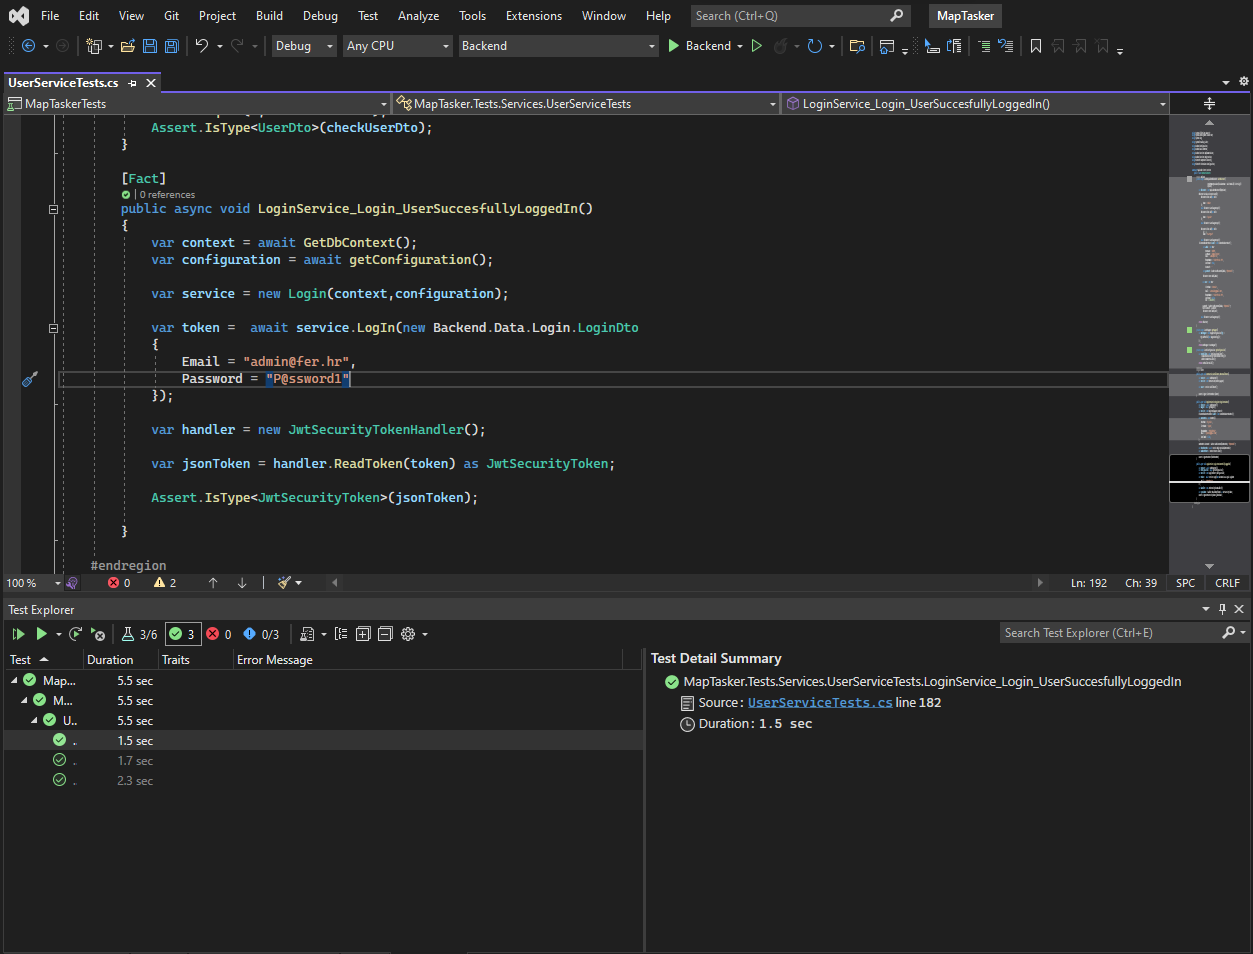
\includegraphics[width=\linewidth]{./slike/Testovi/Unit/UnitTest_3.png}
				\caption{UserSuccesfullyLoggedIn Test}
			\end{figure}
			
			\eject
			
			\noindent \textbf{Ispitni slučaj 4: Dohvaćanje svih prijava nestanka}
			
			\noindent \textbf{Ulaz:}
			
			\begin{packed_enum}
				
				\item Stvaranje novog generatora Id-a
				\item Kreiranje novog MissingReport Servicea
				\item Dohvaćanje svih prijava nestanaka metodom GetAllMissingReports
				
			\end{packed_enum}
			
			\noindent \textbf{Očekivani izlaz:}
			
			\begin{packed_enum}
				
				\item Stvara se generator Id-a
				\item Uspješno kreiranje MissingReporta
				\item Uspješno se dohvaćaju sve prijave nestanaka
				\item Rezultat testa je ispravan
				
			\end{packed_enum}
			
			\noindent \textbf{Izlaz:} Test je zadovoljen. Aplikacija je prošla test.
			
			\begin{figure}[H] 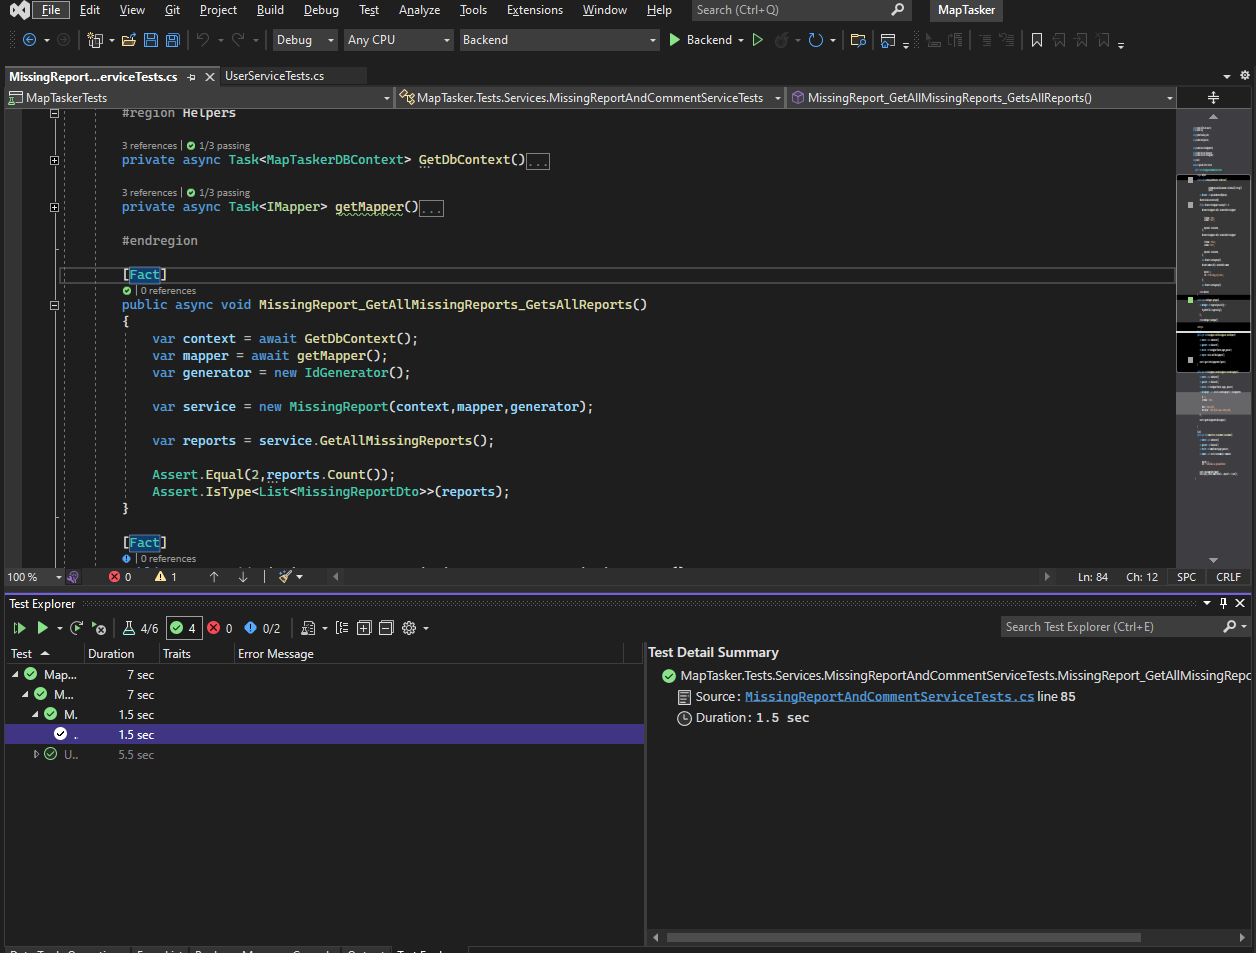
\includegraphics[width=\linewidth]{./slike/Testovi/Unit/UnitTest_4.png}
				\caption{GetAllMissingReports Test}
			\end{figure}
			
			\eject
			
			\noindent \textbf{Ispitni slučaj 5: Stvaranje prijave nestanka}
			
			\noindent \textbf{Ulaz:}
			
			\begin{packed_enum}
				
				\item Stvaranje novog generatora Id-a
				\item Kreiranje MissingReport Servicea
				\item Instanciranje prijave nestanka
				
			\end{packed_enum}
			
			\noindent \textbf{Očekivani izlaz:}
			
			\begin{packed_enum}
				
				\item Stvara se generator Id-a
				\item Uspješno kreiranje MissingReport Servicea
				\item Prijava nestanka uspješno je instancirana
				\item Rezultat testa je ispravan
				
			\end{packed_enum}
			
			\noindent \textbf{Izlaz:} Test je zadovoljen. Aplikacija je prošla test.
			
			\begin{figure}[H] 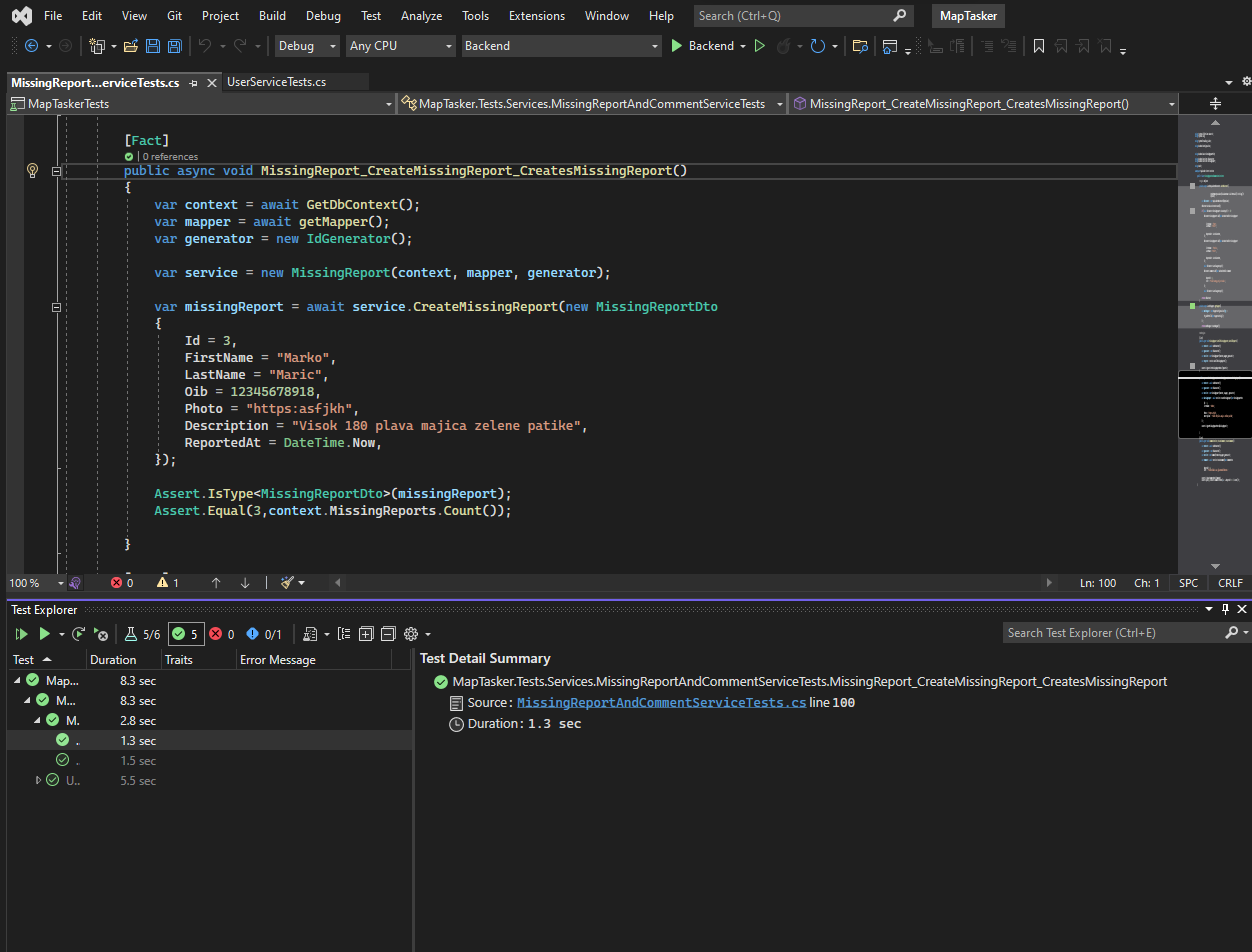
\includegraphics[width=\linewidth]{./slike/Testovi/Unit/UnitTest_5.png}
				\caption{CreatesMissingReport Test}
			\end{figure}
			
			\eject
			
			\noindent \textbf{Ispitni slučaj 6: Kreiranje komentara}
			
			\noindent \textbf{Ulaz:}
			
			\begin{packed_enum}
				
				\item Stvaranje novog generatora Id-a
				\item Kreiranje Comment Servicea
				\item Instanciranje novog komentara
				
			\end{packed_enum}
			
			\noindent \textbf{Očekivani izlaz:}
			
			\begin{packed_enum}
				
				\item Stvara se generator Id-a
				\item Uspješno se kreiran Comment Service
				\item Komentar je uspješno instanciran
				\item Rezultat testa je ispravan
				
			\end{packed_enum}
			
			\noindent \textbf{Izlaz:} Test je zadovoljen. Aplikacija je prošla test.
			
			\begin{figure}[H] 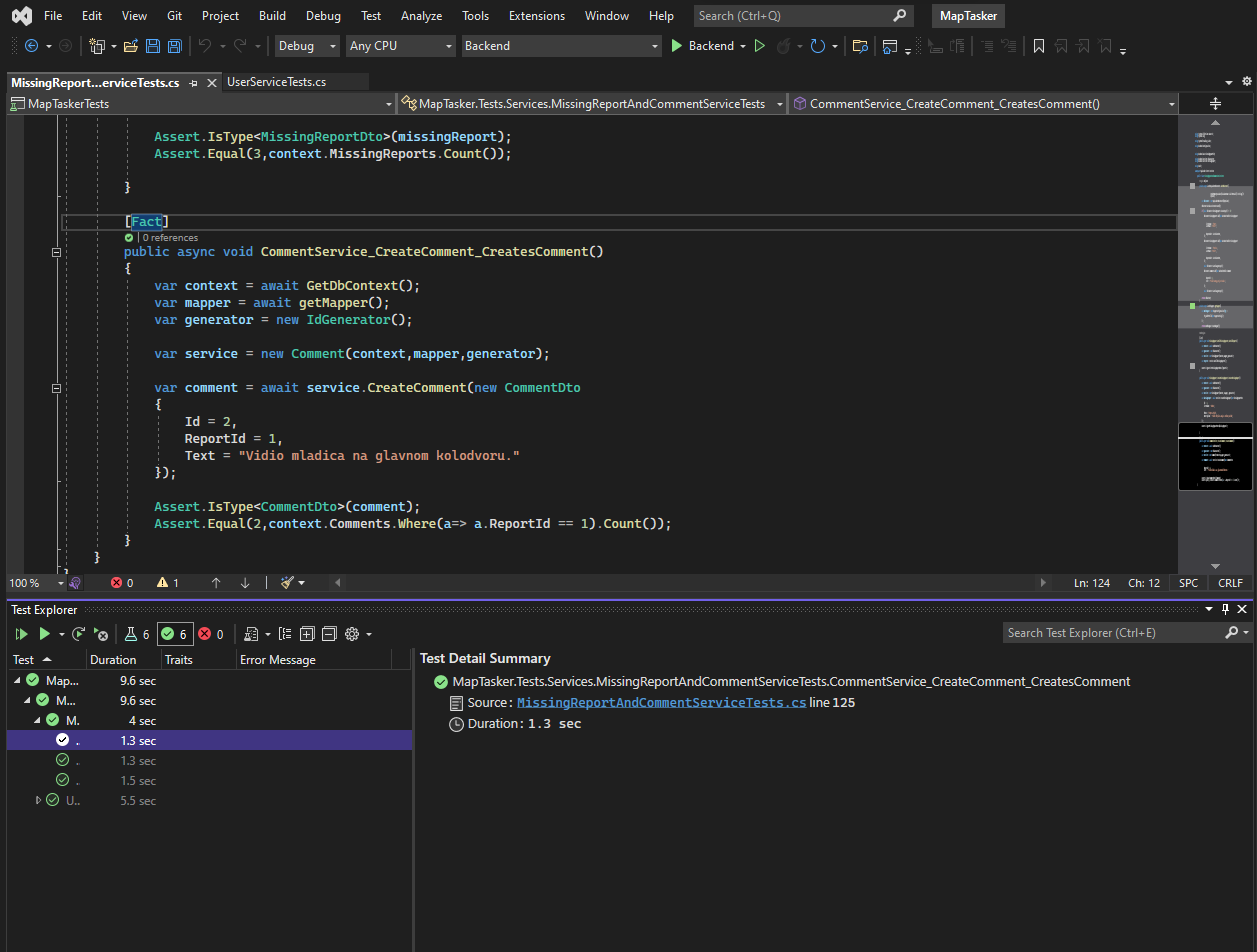
\includegraphics[width=\linewidth]{./slike/Testovi/Unit/UnitTest_6.png}
				\caption{CreatesComments Test}
			\end{figure}
			
			\eject
			
			
			
			\subsection{Ispitivanje sustava}
			
			\par
			Svi Selenium testovi izvršeni su automatski. Ispitivanje je provedeno po obrascima uporabe. Ispitani su obrasci uporabe:
			
			\begin{packed_enum}
				
				\item UC1 - Registracija u sustav
				\item UC2 - Prijava u sustav
				\item UC4 - Prijava nestale osobe
				\item UC5 - Komentiranje prijave nestale osobe
				
			\end{packed_enum}
		
			
			\noindent \textbf{Ispitni slučaj 1: Registracija}
			
			\noindent \textbf{Ulaz:}
			
			\begin{packed_enum}
				
				\item Učitavanje početne stranice i namještanje veličine prozora
				\item Pritisak na gumb "Register"
				\item Korisnik unosi tražene podatke te odabire ulogu koju želi
				
			\end{packed_enum}
			
			\noindent \textbf{Očekivani izlaz:}
			
			\begin{packed_enum}
				
				\item Početna stranica uspješno se učitava
				\item Učitavanje forme za registraciju
				\item Korisnik prima obavijest o uspješno obavljenoj registraciji
				\item Rezultat testa je ispravan
				
			\end{packed_enum}
			
			\noindent \textbf{Izlaz:} Test je zadovoljen. Aplikacija je prošla test.
			
			\begin{figure}[H] 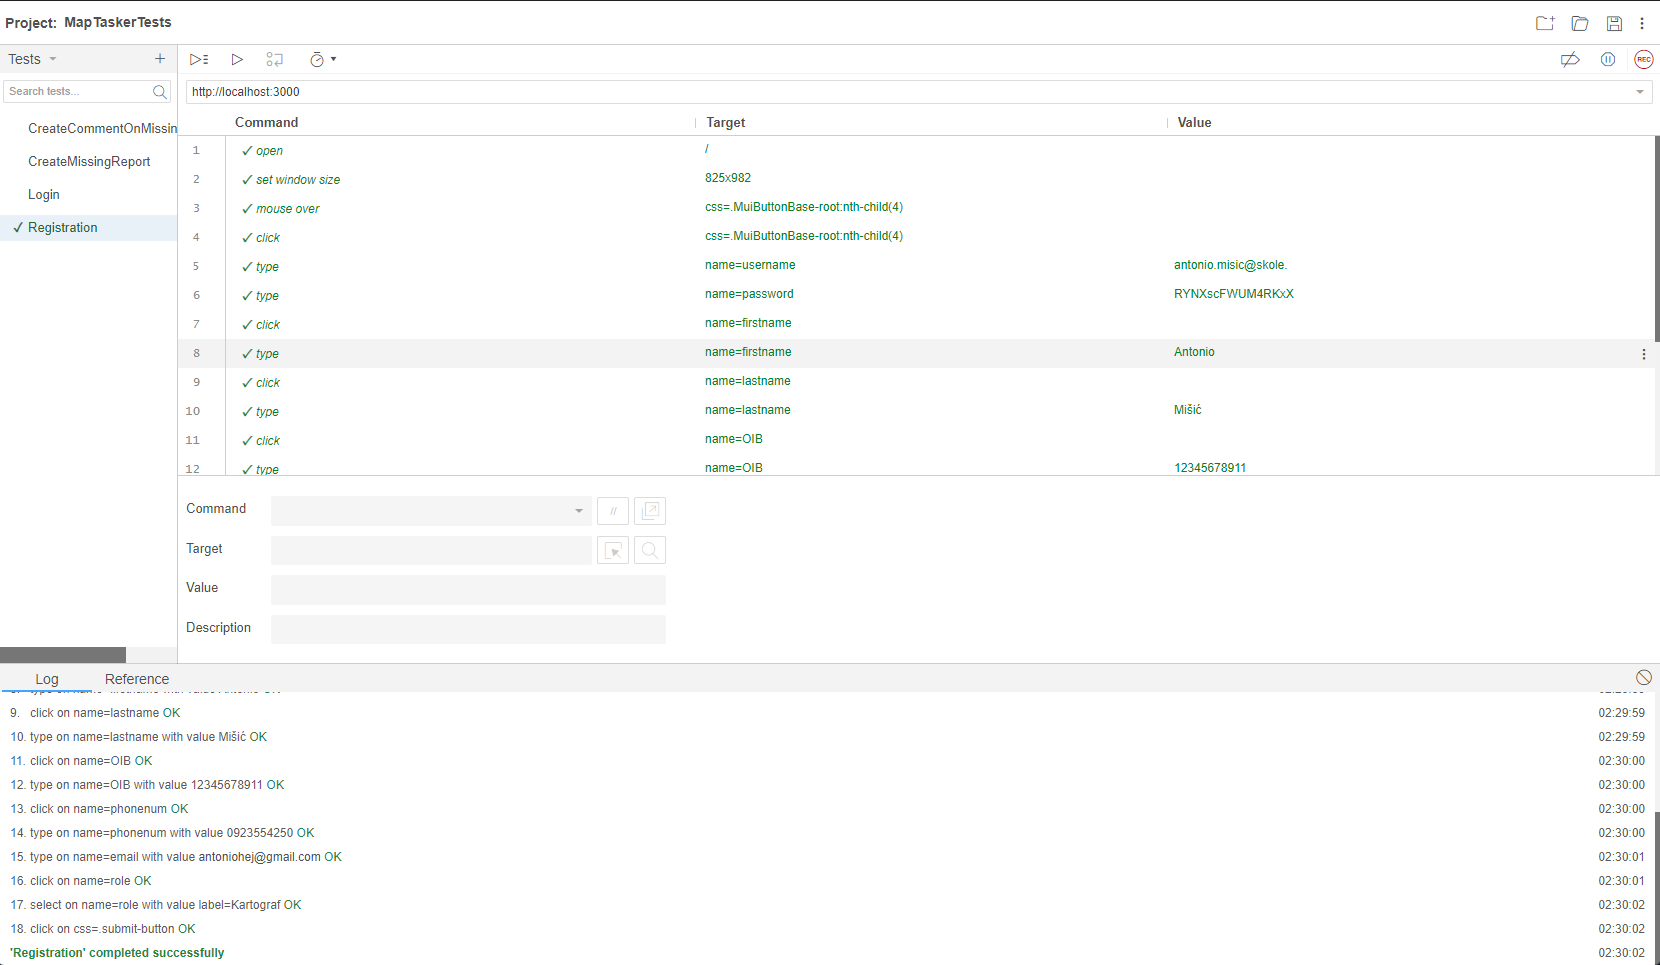
\includegraphics[width=\linewidth]{./slike/Testovi/Selenium/Selenium_1.png}
				\caption{Registration Test}
			\end{figure}
			
			\eject
			
			\noindent \textbf{Ispitni slučaj 2: Prijava}
			
			\noindent \textbf{Ulaz:}
			
			\begin{packed_enum}
				
				\item Učitavanje početne stranice i namještanje veličine prozora
				\item Pritisak na gumb "Login"
				\item Korisnik unosi e-mail adresu i lozinku
				
			\end{packed_enum}
			
			\noindent \textbf{Očekivani izlaz:}
			
			\begin{packed_enum}
				
				\item Početna stranica uspješno se učitava
				\item Učitavanje forme za prijavu
				\item Korisnik je uspješno prijavljen u sustav
				\item Rezultat testa je ispravan
				
			\end{packed_enum}
			
			\noindent \textbf{Izlaz:} Test je zadovoljen. Aplikacija je prošla test.
			
			\begin{figure}[H] 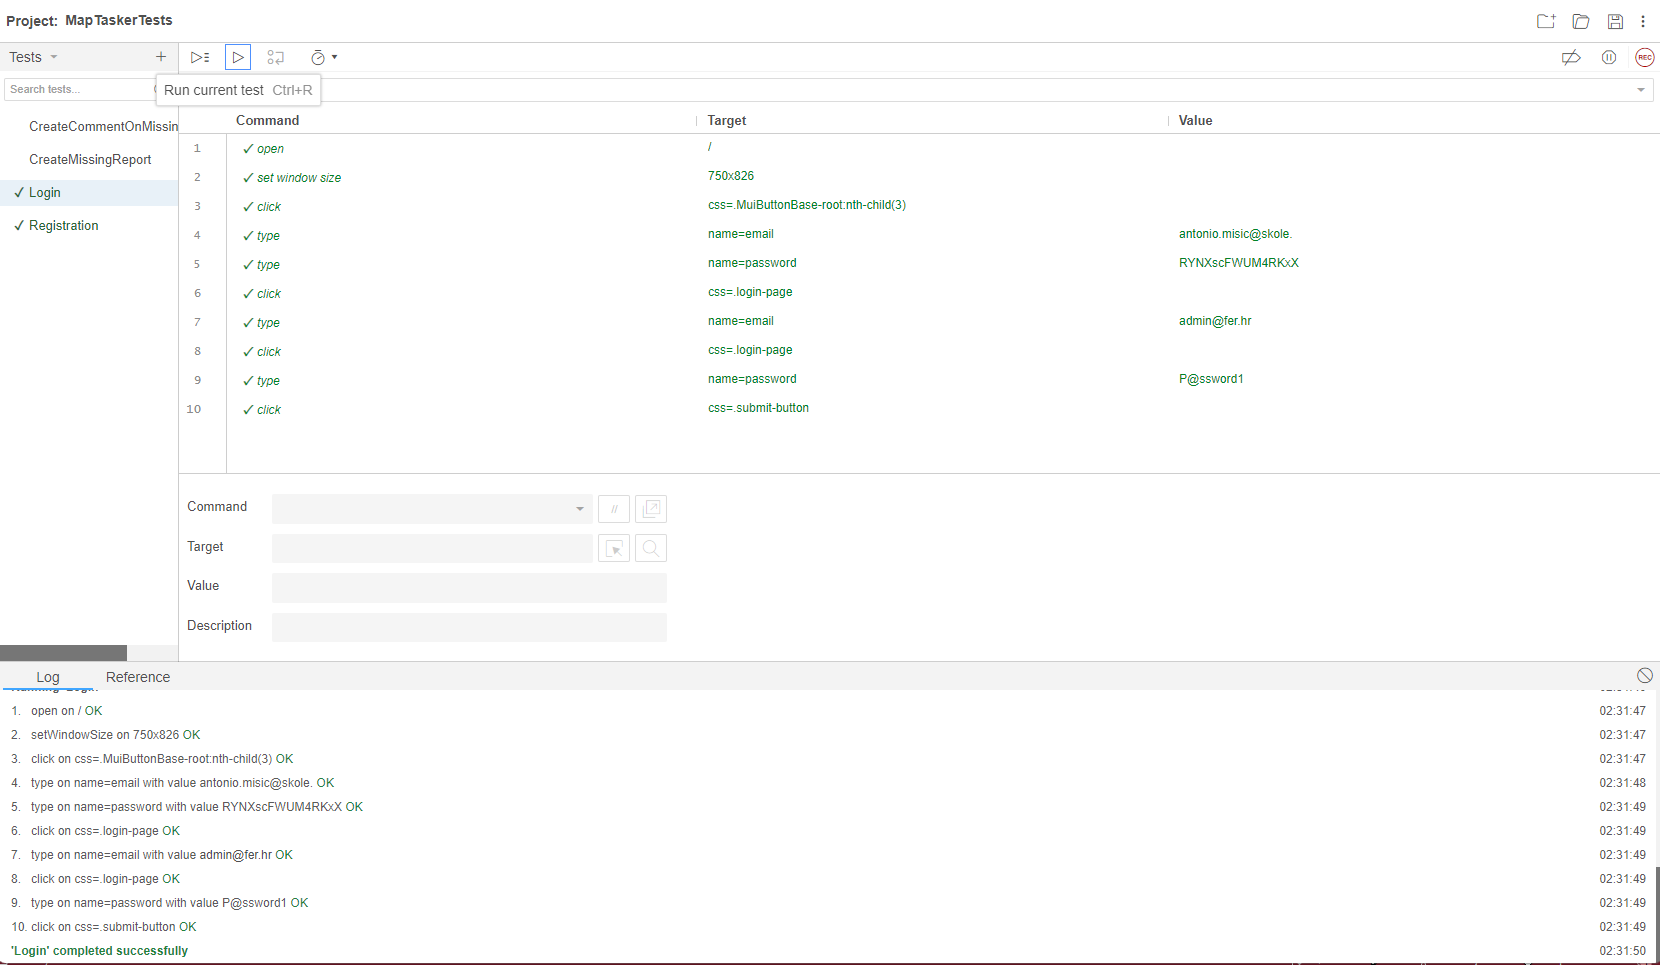
\includegraphics[width=\linewidth]{./slike/Testovi/Selenium/Selenium_2.png}
				\caption{Login Test}
			\end{figure}
			
			\eject
			
			\noindent \textbf{Ispitni slučaj 3: Kreiranje prijave nestanka}
			
			\noindent \textbf{Ulaz:}
			
			\begin{packed_enum}
				
				\item Učitavanje početne stranice i namještanje veličine prozora
				\item Pritisak na gumb "Prijavi"
				\item Unošenje podataka o nestaloj osobi
				
			\end{packed_enum}
			
			\noindent \textbf{Očekivani izlaz:}
			
			\begin{packed_enum}
				
				\item Početna stranica uspješno se učitava
				\item Učitavanje forme za prijavu nestanka osobe
				\item Obavijest o uspješnoj prijavi nestale osobe
				\item Rezultat testa je ispravan
				
			\end{packed_enum}
			
			\noindent \textbf{Izlaz:} Test je zadovoljen. Aplikacija je prošla test.
			
			\begin{figure}[H] 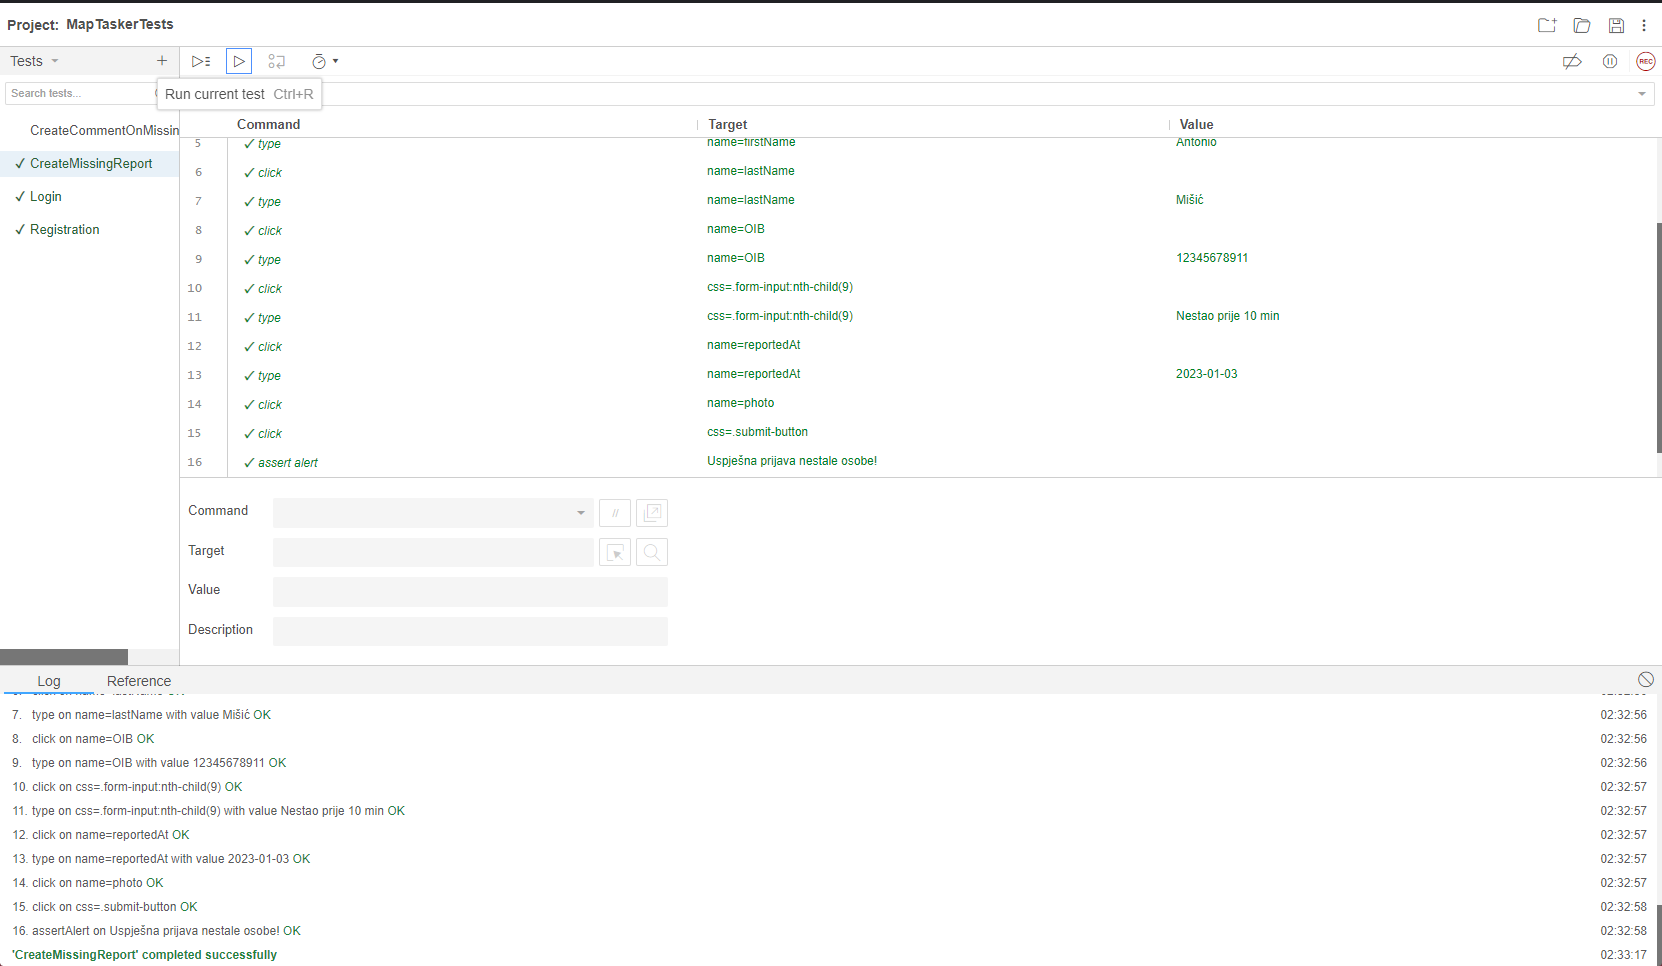
\includegraphics[width=\linewidth]{./slike/Testovi/Selenium/Selenium_3.png}
				\caption{CreateMissingReport Test}
			\end{figure}
			
			\eject
			
			\noindent \textbf{Ispitni slučaj 4: Kreiranje komentara na prijavu nestanka}
			
			\noindent \textbf{Ulaz:}
			
			\begin{packed_enum}
				
				\item Učitavanje početne stranice i namještanje veličine prozora
				\item Pritisak na gumb "Nestale osobe"
				\item Stvaranje komentara kraj nestale osobe
				
			\end{packed_enum}
			
			\noindent \textbf{Očekivani izlaz:}
			
			\begin{packed_enum}
				
				\item Početna stranica uspješno se učitava
				\item Učitavanje stranice s nestalim osobama
				\item Komentar je prikazan na stranici
				\item Rezultat testa je ispravan
				
			\end{packed_enum}
			
			\noindent \textbf{Izlaz:} Test je zadovoljen. Aplikacija je prošla test.
			
			\begin{figure}[H] 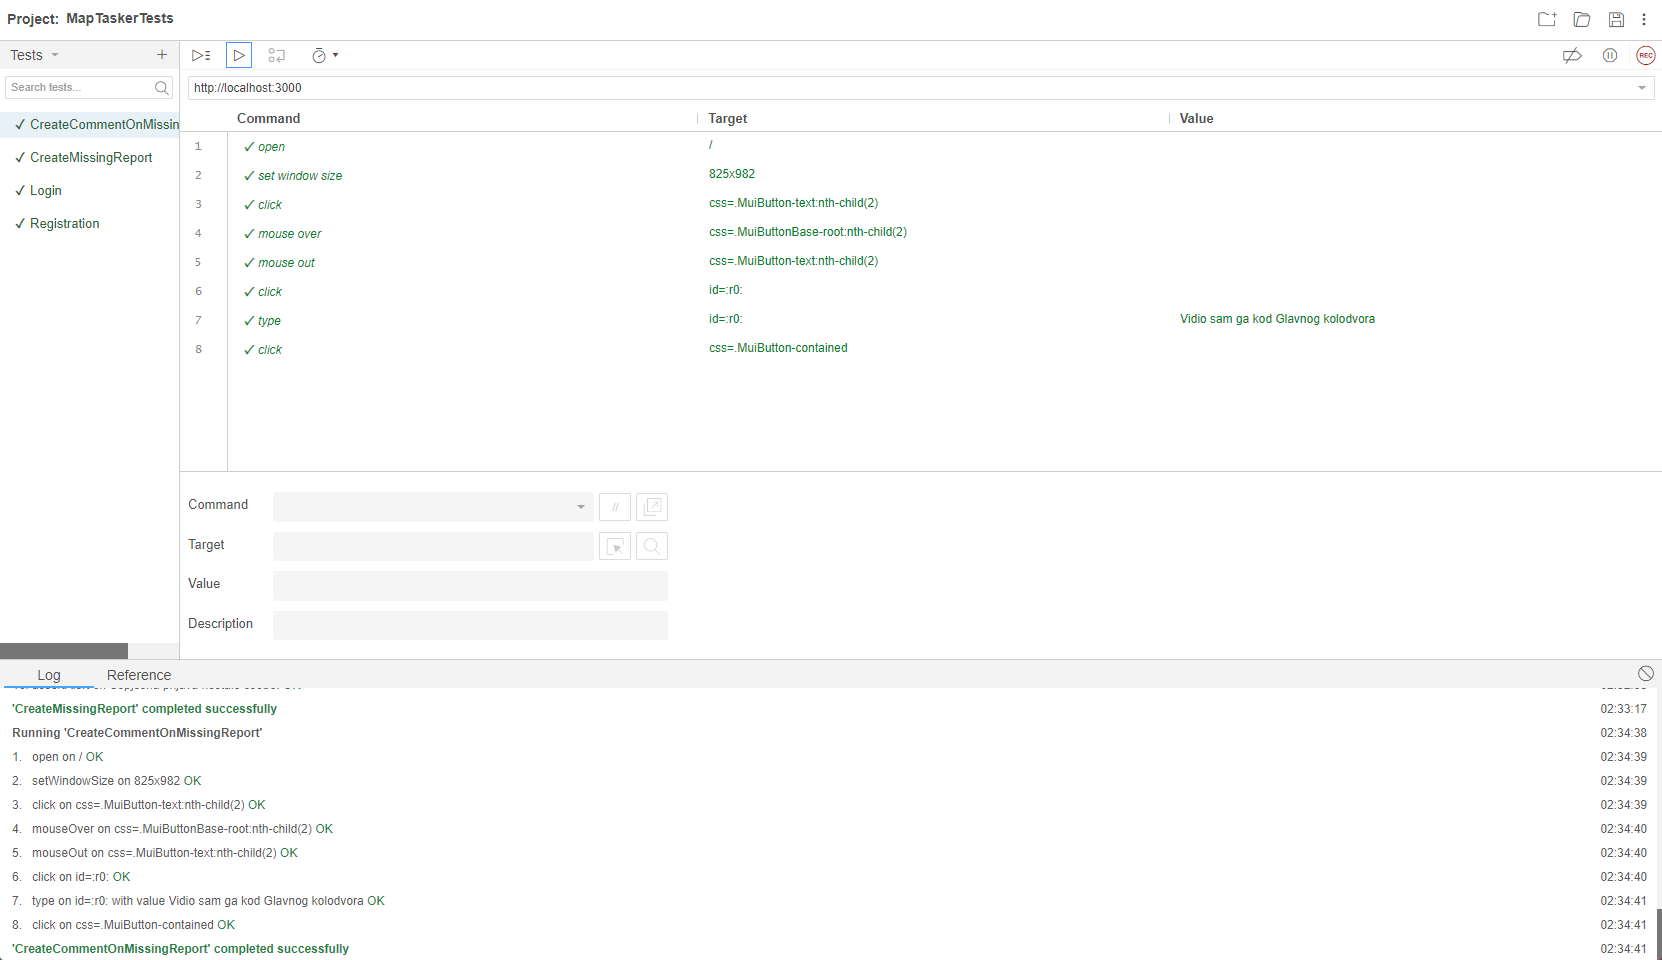
\includegraphics[width=\linewidth]{./slike/Testovi/Selenium/Selenium_4.png}
				\caption{CreateComment Test}
			\end{figure}
			
			\eject
		
		
		\section{Dijagram razmještaja}
						
		Korisnik se sa svog uređaja spaja na poslužiteljsko računalo HTTP protokolom. Na računalu se nalazi web aplikacija čiji se \textit{backend} i \textit{baza podataka} postavljeni na Azure serveru dok se \textit{frontend} nalazi na Vercel serveru.
            
			\begin{figure}[H]
					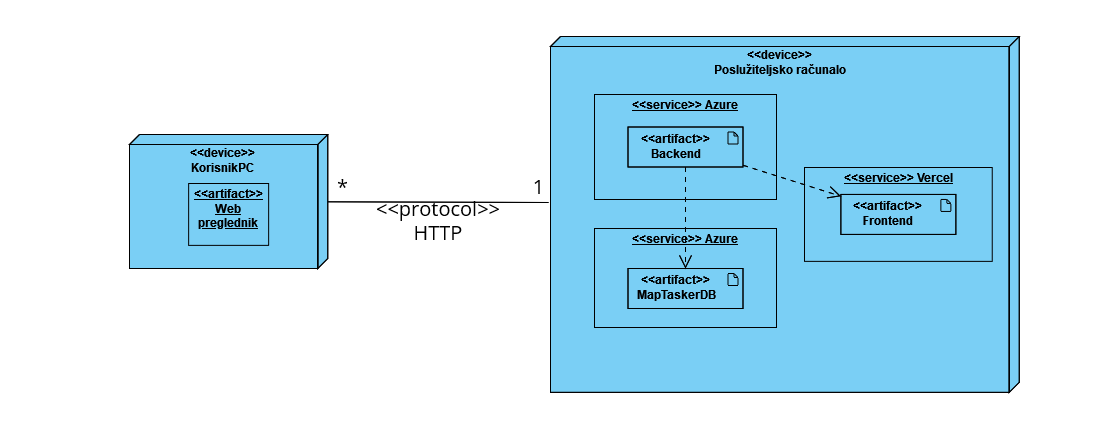
\includegraphics[scale=0.55]{dijagrami/DijagramRazm.png} %veličina slike u odnosu na originalnu datoteku i pozicija slike
					\centering
					\caption{Dijagram razmještaja}
					\label{fig:promjene}
			\end{figure}

			\eject
		
		\section{Upute za puštanje u pogon}

		
			\textbf{Prijava u Azure račun}
			
			\noindent Korisnik se treba prijaviti u svoj Microsoft Azure račun.
			
			\vspace{10mm}
			
			\noindent\textbf{Stvaranje baze podataka na Azure serveru}
	
			\noindent Nakon prijave, korisnik treba u izborniku odabrati opciju "Create a resource", te od ponuđenih odabrati "SQL Database".
	
			\vspace{10mm}
		
			\begin{figure}[H]
				 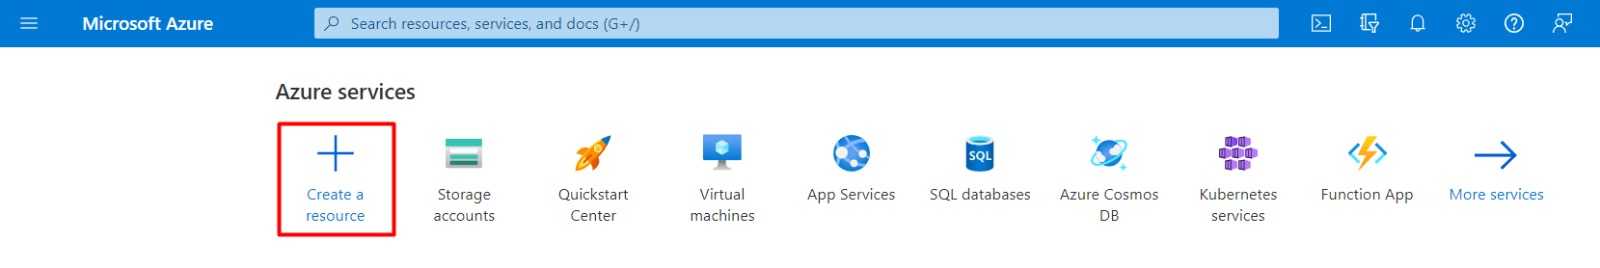
\includegraphics[width=\linewidth]{./slike/baza0.jpg}
				  \centering
				  \caption{Odabir opcije "Create a resource"}
			  \end{figure}
	
			\vspace{20mm}
			
		
			\begin{figure}[H]
				 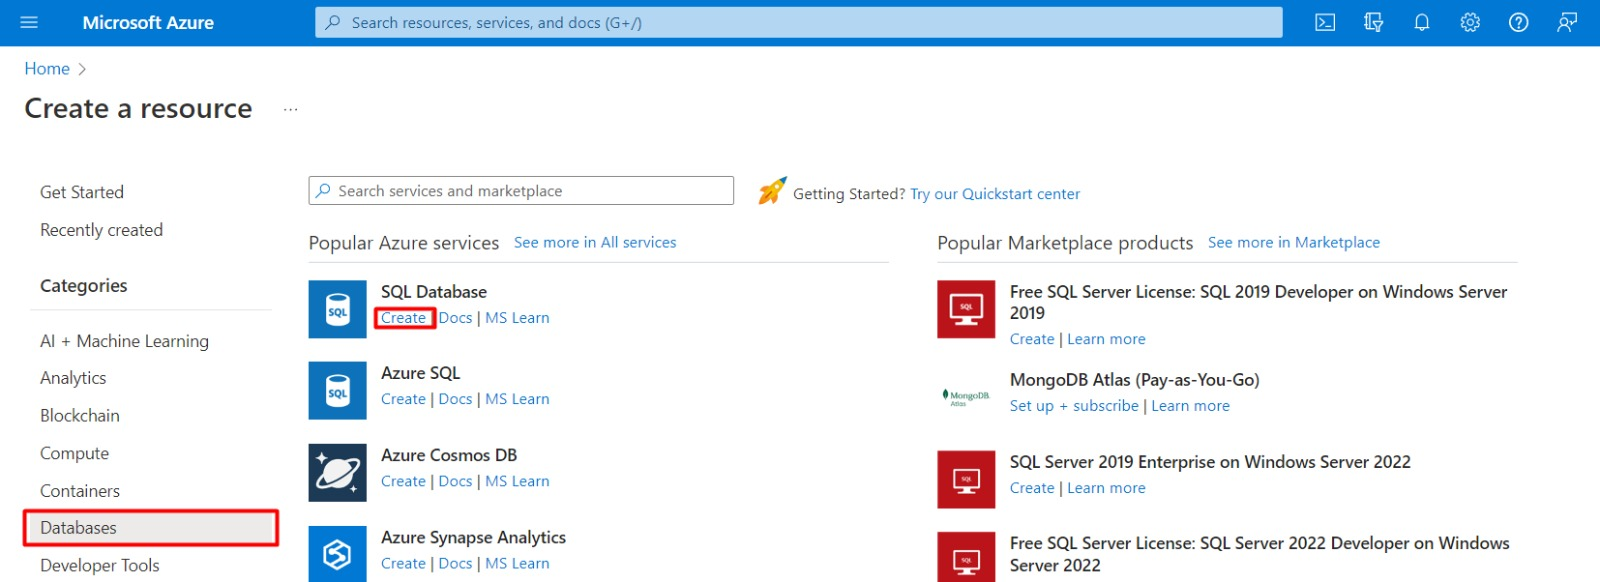
\includegraphics[width=\linewidth]{./slike/baza1.jpg}
				  \centering
				  \caption{Odabir opcije "SQL Database"}
			  \end{figure}
			  
		
		\vspace{25mm}
	
			\noindent Korisnik treba dati ime bazi, napraviti njezin resource group i server. Također potrebno je odabrati i pricing tier, odnosno cjenovni rang koji ovisi o željenim performansama.
		
			\vspace{10mm}
	
			\begin{figure}[H]
				 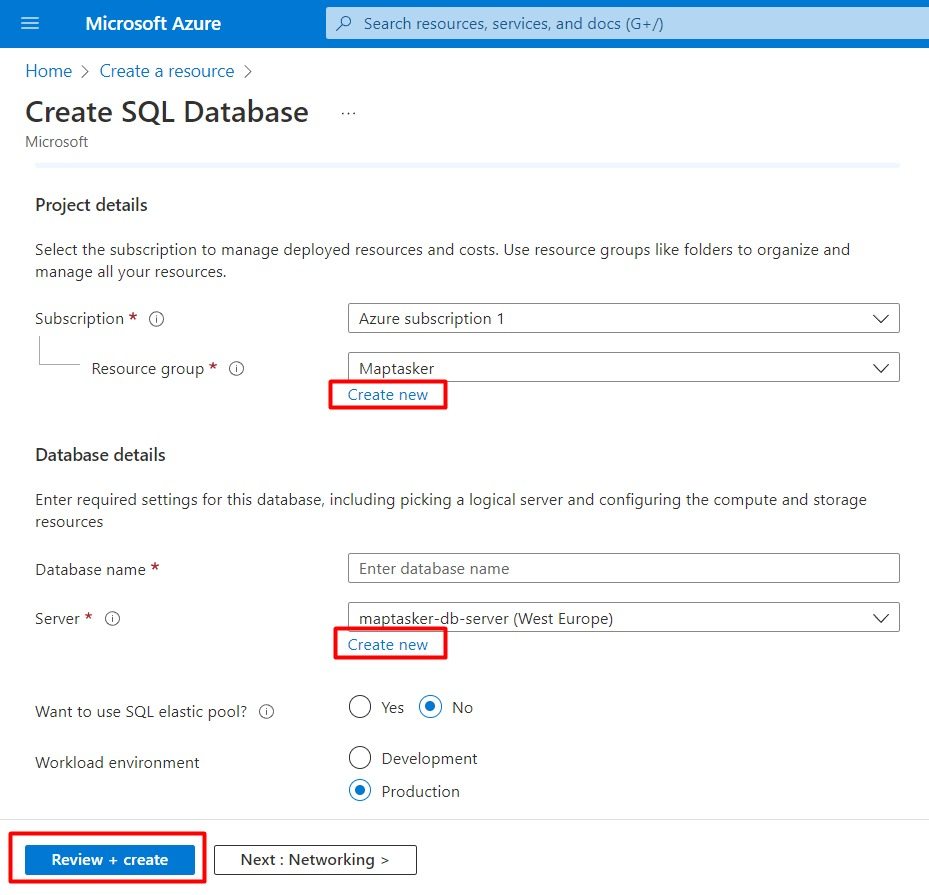
\includegraphics[width=\linewidth]{./slike/baza2.jpg}
				  \centering
				  \caption{Dodavanje željenih svojstava bazi}
			  \end{figure}
	
			
			\vspace{5mm}
	
			\noindent Potrebno je otvoriti Azure Data Studio i spojiti se na lokalni server, zatim desnim klikom na lokalnu bazu na padajućem izborniku odabrati opciju "Data-tier Application Wizard". Nakon toga korisnik treba označiti zadnju navedenu operaciju ("Export the schema..." ), kliknuti Next, te na kraju odabrati lokaciju kreirane .bacpac datoteke i pričekati dok se datoteka ne stvori.
	
	
			\vspace{10mm}
	
			\begin{figure}[H]
				 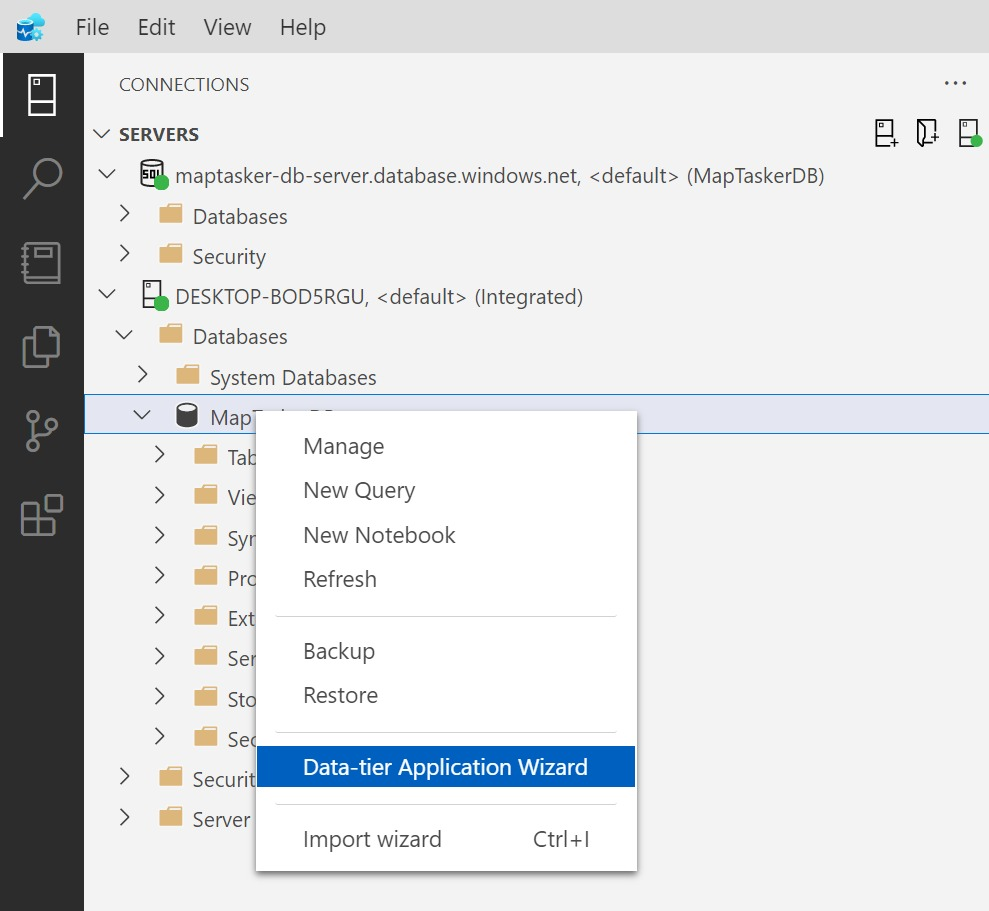
\includegraphics[width=\linewidth]{./slike/baza3.jpg}
				  \centering
				  \caption{Odabir opcije "Data-tier Application Wizard"}
			  \end{figure}
	
			\vspace{25mm}
	
			\begin{figure}[H]
				 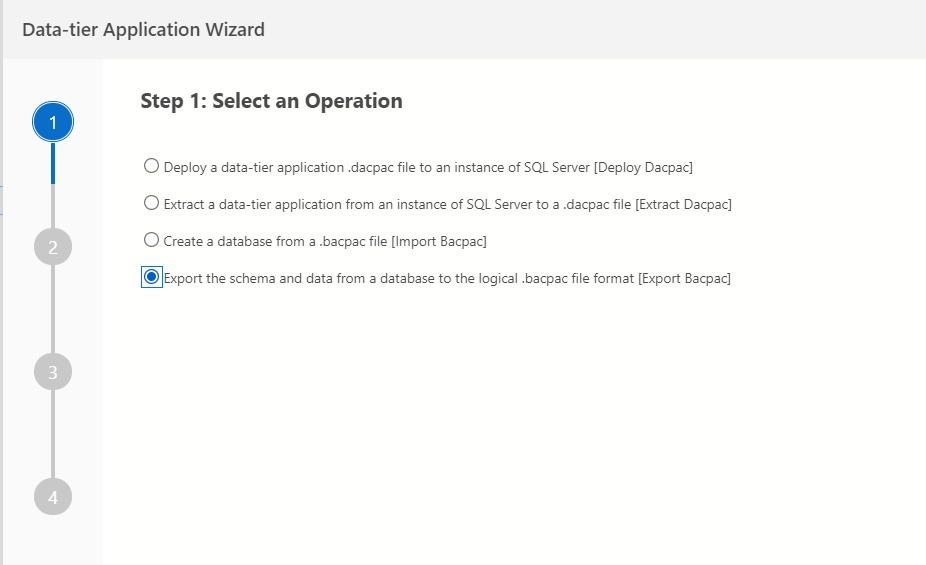
\includegraphics[width=\linewidth]{./slike/baza4.jpg}
				  \centering
				  \caption{Odabir željene operacije}
			  \end{figure}
			
			\vspace{15mm}
	
			\noindent Na kraju je potrebno spojiti se na Azure server i ponovno otvoriti "Data-tier Application Wizard". Zatim korisnik treba odabrati opciju "Create a database" kojom će stvoriti bazu, pratiti daljne korake i odabrati prethodno stvoreni .bacpac file.
	
			\vspace{10mm}
	
			\begin{figure}[H]
				 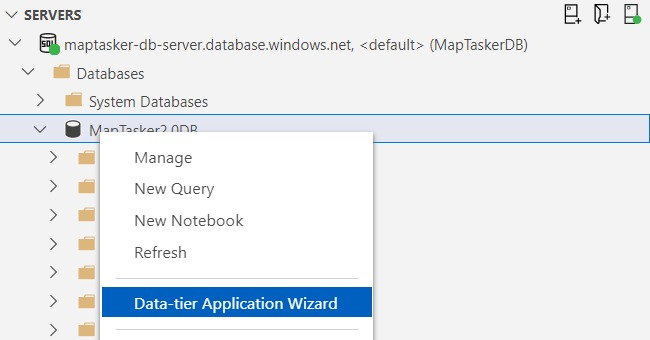
\includegraphics[width=\linewidth]{./slike/baza5.jpg}
				  \centering
				  \caption{Odabir opcije "Data-tier Application Wizard"}
			  \end{figure}
	
			\vspace{10mm}
	
			\begin{figure}[H]
				 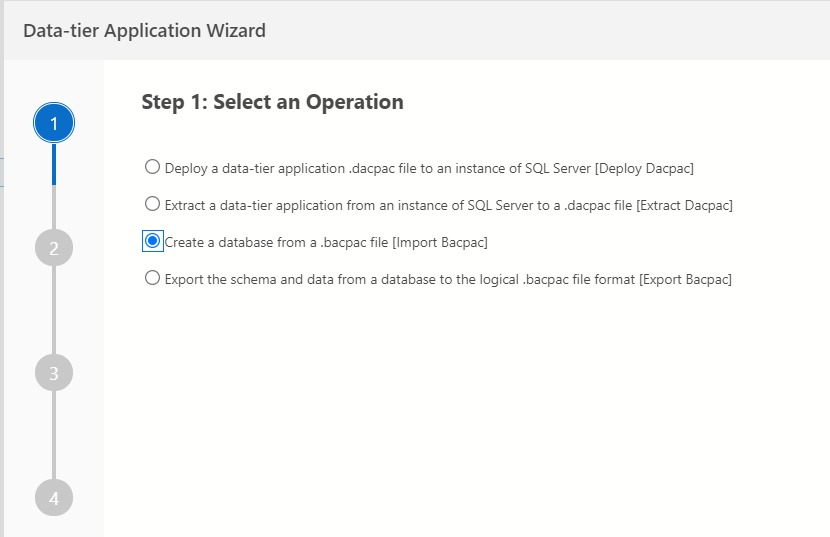
\includegraphics[width=\linewidth]{./slike/baza6.jpg}
				  \centering
				  \caption{Odabir operacije stvaranja baze}
			  \end{figure}
	
			\noindent\textbf{Stvaranje backend API-ja na Azure serveru}
	
			\noindent Za početak, potrebno je otvoriti projekt u Visual Studiu, i desnim klikom na Backend projekt u padajućem izborniku odabrati opciju "Publish". Zatim se preko grafičkog sučelja ulogirati u Azure i označiti isti resource group kao i za bazu.
	
			\vspace{10mm}
	
			\begin{figure}[H]
				 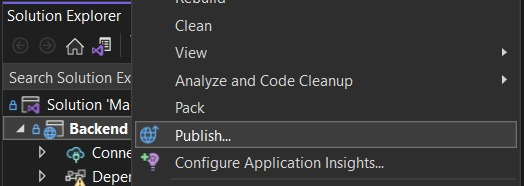
\includegraphics[width=\linewidth]{./slike/backend1.jpg}
				  \centering
				  \caption{Odabir opcije "Publish"}
			  \end{figure}
			  
			\vspace{10mm}
	
			\noindent Za ispravno pokretanje backenda, potrebno je otići u Azure na novonastali App Service u Configuration sučelje. Potrebno je dodati novi Application Setting naziva CONNECTION\_STRING i vrijednosti connection stringa dobivenog iz Azure postavka za bazu. Ponoviti postupak umetanja connection stringa za podizbornik Connection String, ovoga puta s nazivom ConnectionString. 
	
			\vspace{10mm}
	
			\begin{figure}[H]
				 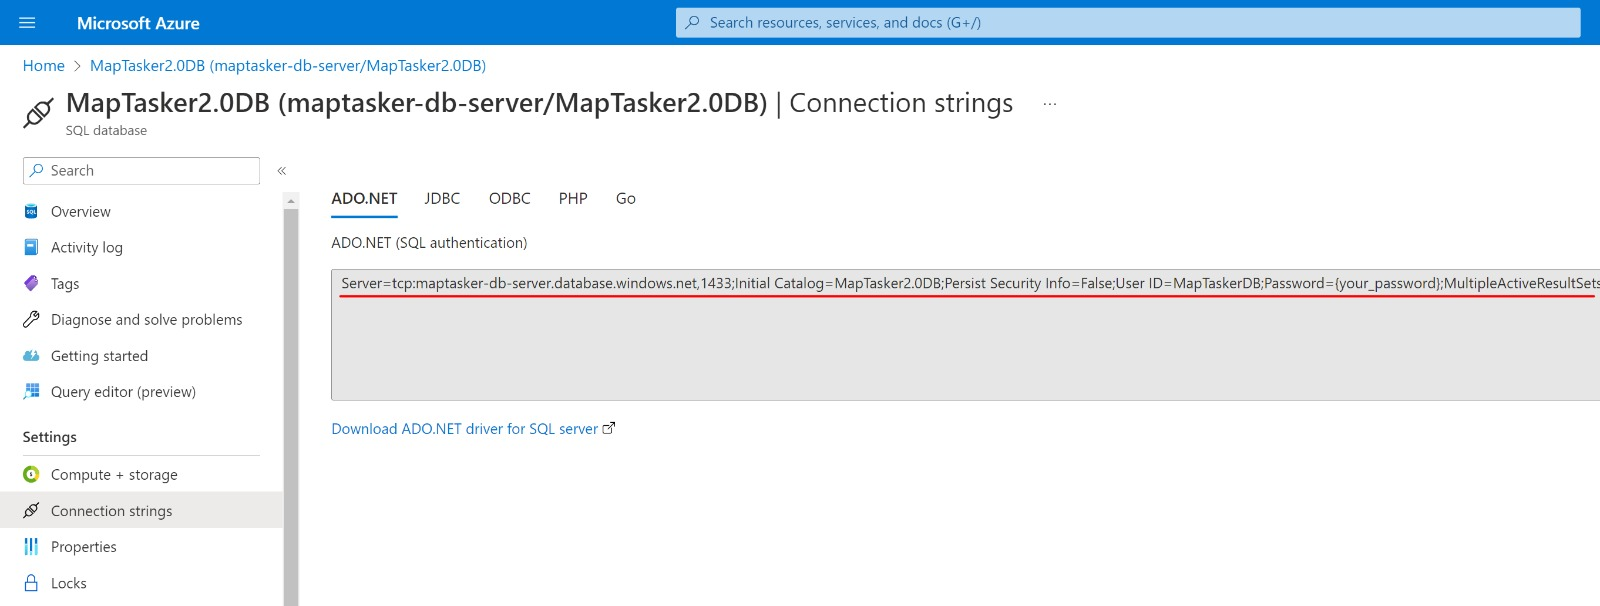
\includegraphics[width=\linewidth]{./slike/backend1a.jpg}
				  \centering
				  \caption{Lokacija vrijednosti connection stringa}
			  \end{figure}
			  
			\vspace{20mm}
	
			\begin{figure}[H]
				 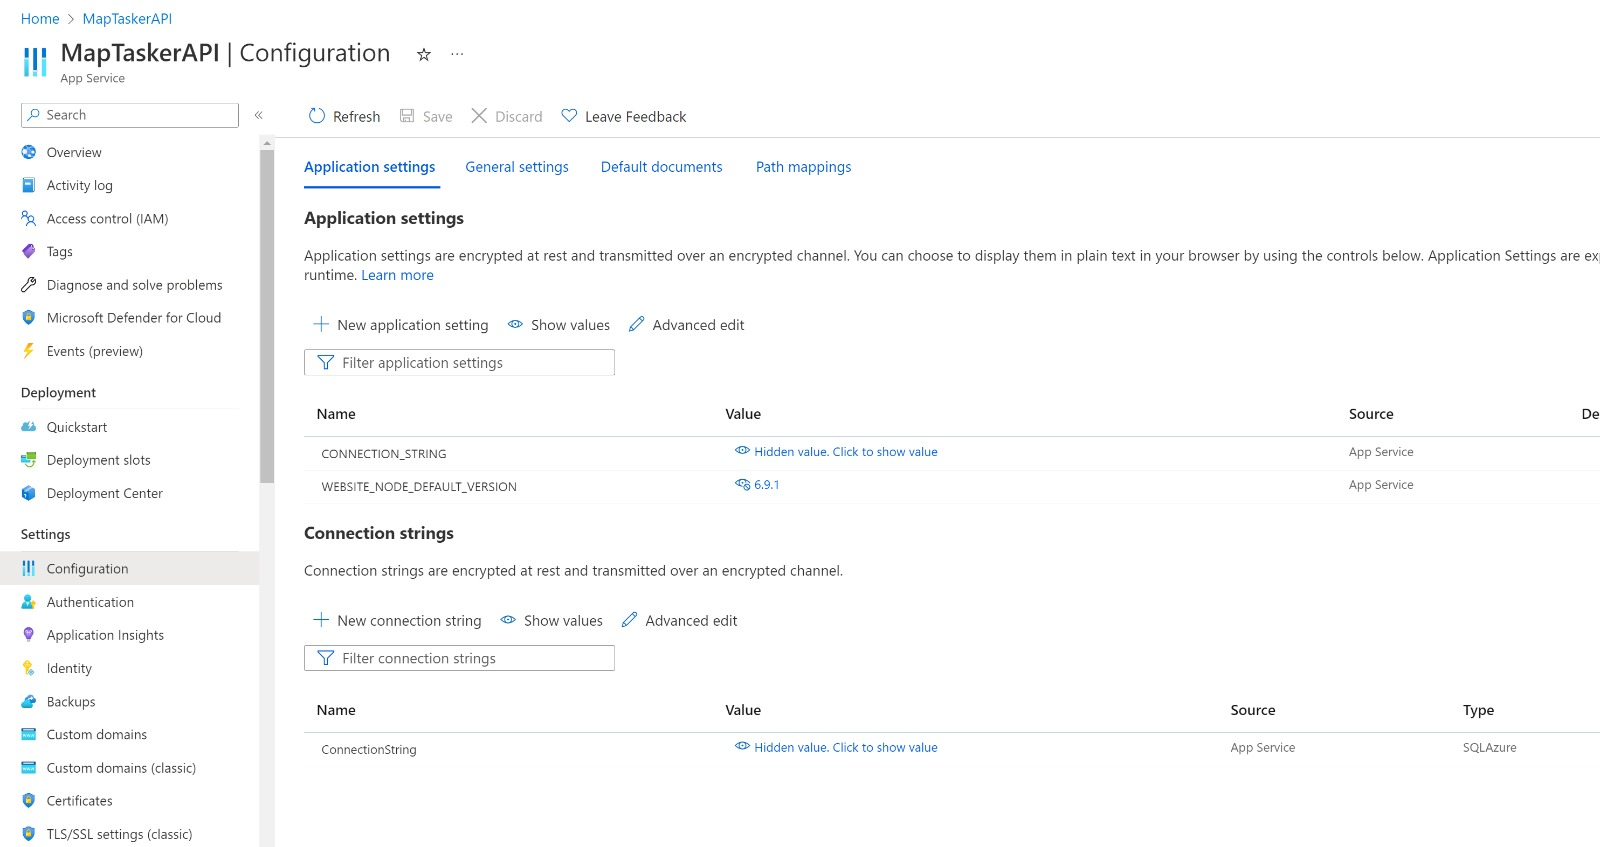
\includegraphics[width=\linewidth]{./slike/backend2.jpg}
				  \centering
				  \caption{Unos vrijednosti connection stringa}
			  \end{figure}
			
			\vspace{30mm}
	
			\noindent\textbf{Stvaranje frontenda aplikacije na Vercel platformi}
	
			\noindent Za početak nužno je uvesti git repozitorij projekta.
	
			\vspace{10mm}
	
			\begin{figure}[H]
				 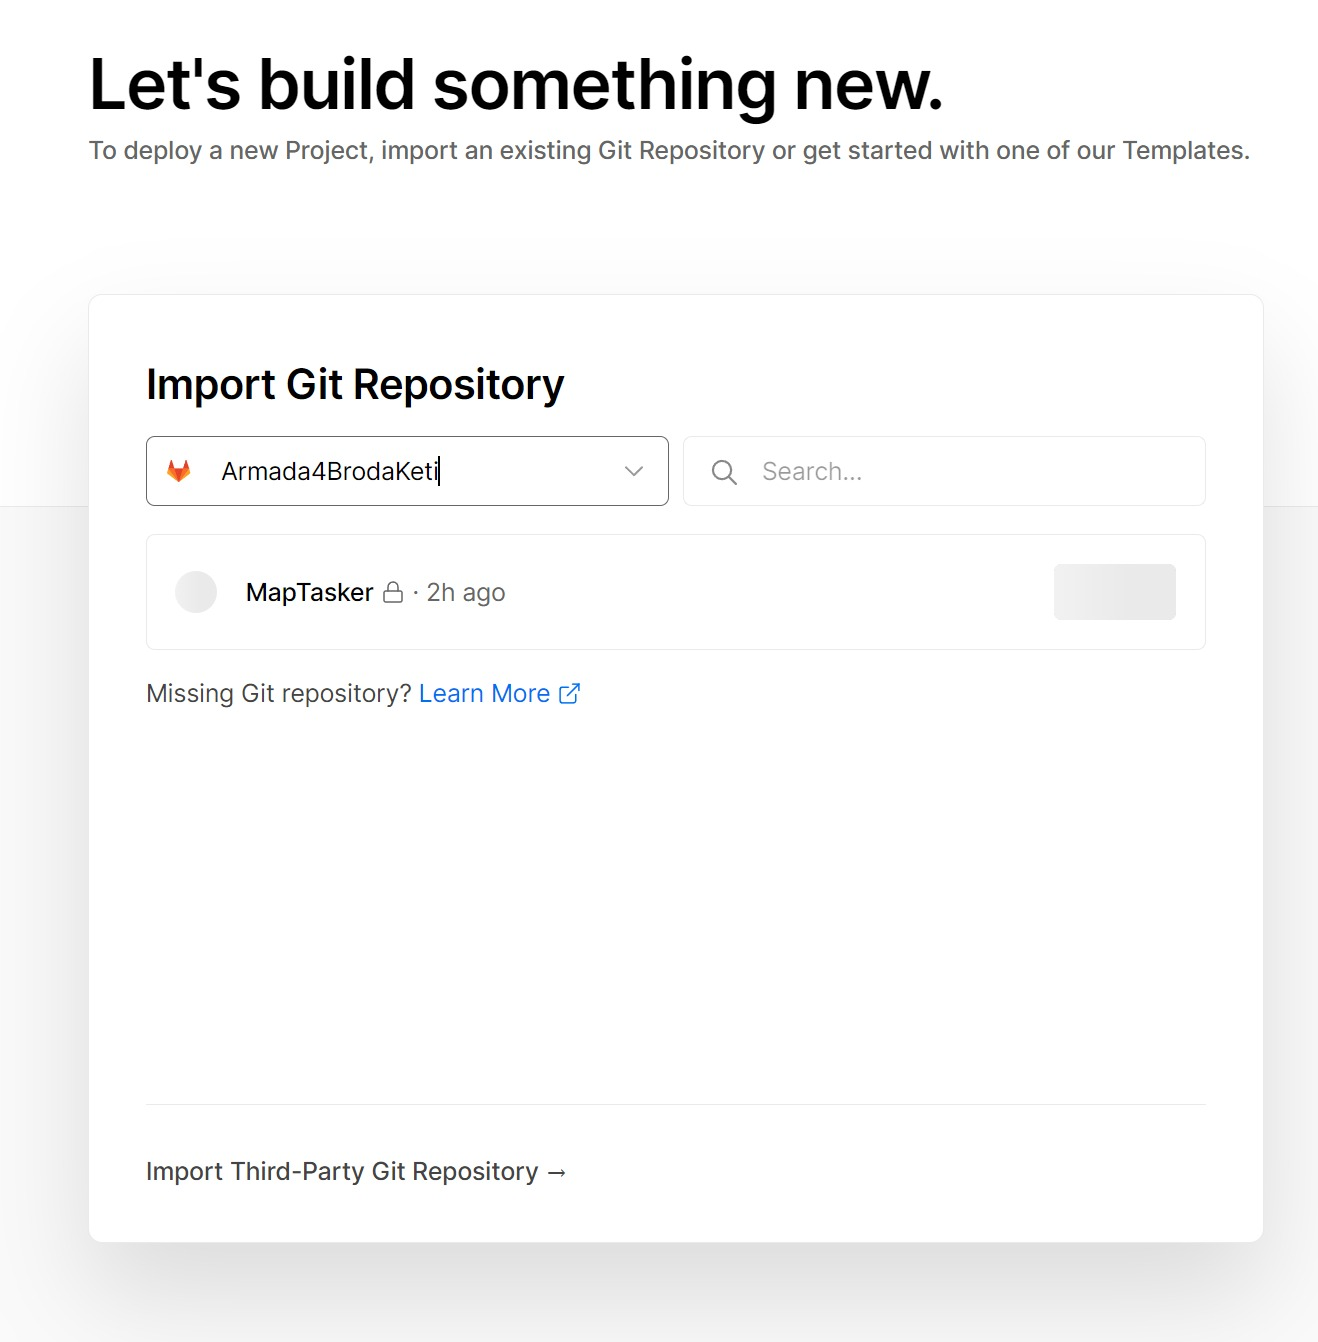
\includegraphics[width=\linewidth]{./slike/front1.jpg}
				  \centering
				  \caption{Uvoz git repozitorija projekta}
			  \end{figure}
	
			\vspace{20mm}
	
			\noindent Nakon toga potrebno je otići u "Build \& Development Settings" sučelje i postaviti naredbe potrebne za pokretanje npm skripti koje su prikazane na slici 5.12.
	
			\vspace{10mm}
	
			\begin{figure}[H]
				 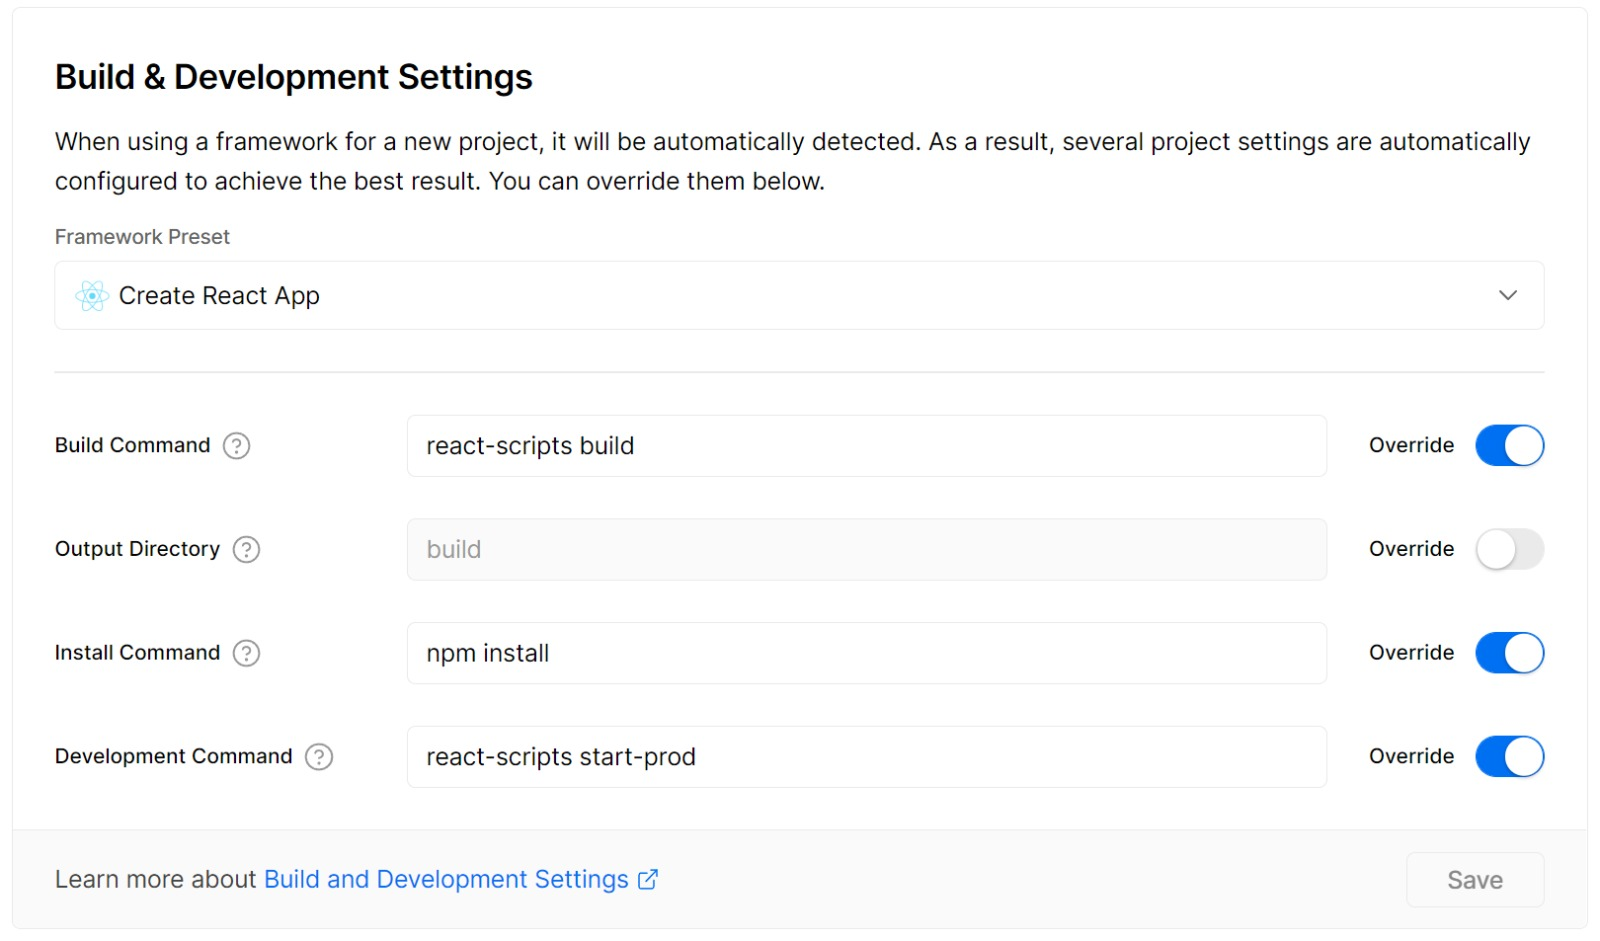
\includegraphics[width=\linewidth]{./slike/front2.jpg}
				  \centering
				  \caption{Naredbe za pokretanje npm skripti}
			  \end{figure}
	
			\vspace{20mm}
	
			\noindent U sučelju "Environment Variables" kopirati link na backend API (vidljiv u Azureu) pod ključem REACT\_APP\_API\_URL.
	
			\vspace{10mm}
	
			\begin{figure}[H]
				 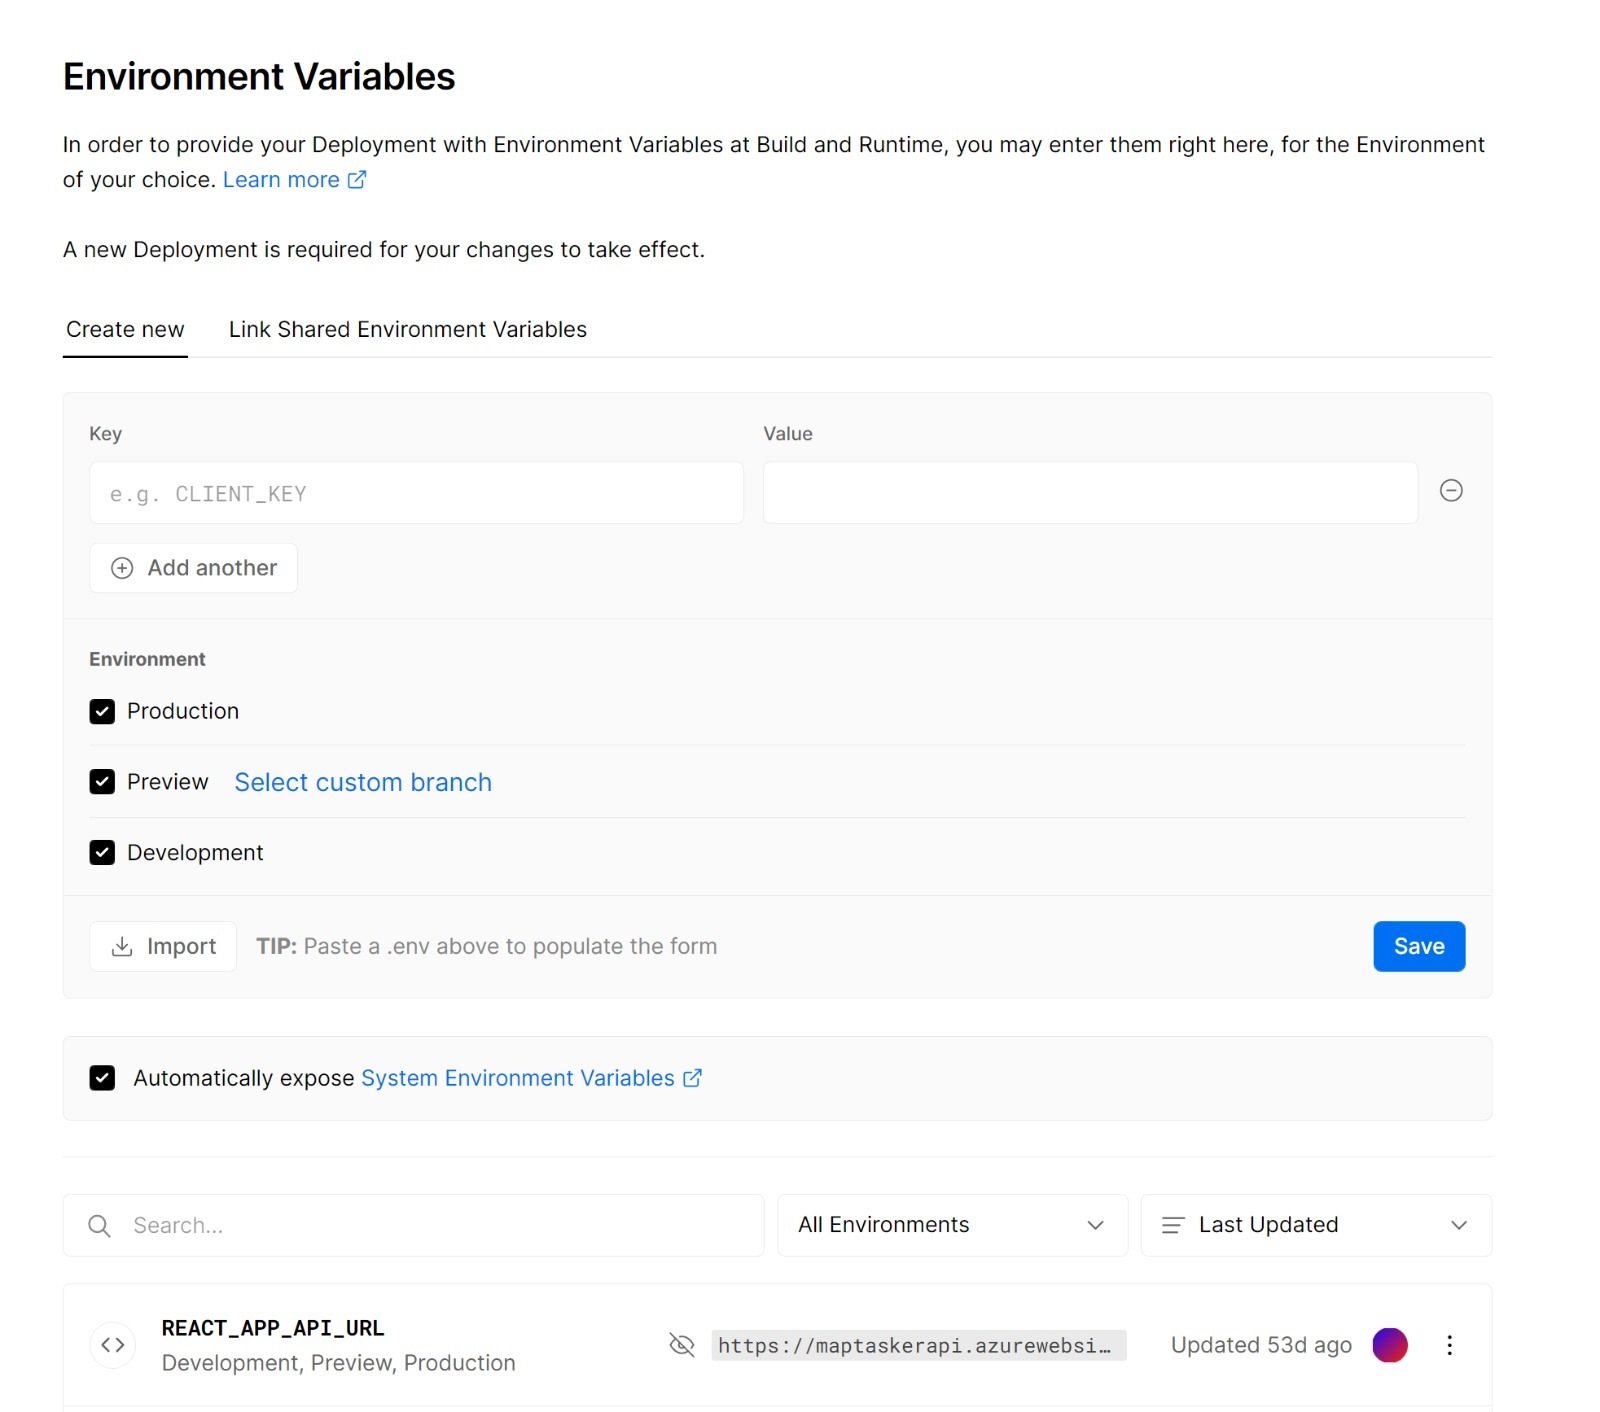
\includegraphics[width=\linewidth]{./slike/front3.jpg}
				  \centering
				  \caption{Podešavanje varijabli okruženja}
			  \end{figure}
	
			  \vspace{20mm}
	
			  \noindent Spremanjem postavki razmještanje frontenda će se dogoditi automatski i ponovno se pokrenuti pushanjem na main branch. 
	\eject 
	

